% !TEX TS-program = pdflatexmk
%% This is an example first chapter.  You should put chapter/appendix that you
%% write into a separate file, and add a line \include{yourfilename} to
%% main.tex, where `yourfilename.tex' is the name of the chapter/appendix file.
%% You can process specific files by typing their names in at the 
%% \files=
%% prompt when you run the file main.tex through LaTeX.
\chapter{Introduction}

\section{The Standard Model}
In the classical view of our physical world, even from the very early phase of human's history of understanding the universe, people have been convinced that all matter is made of some fundamental elements, and studying the elementary structure of the matter along with the interaction between those elements help us better understand the world and innovates the new technologies that deeply changes human society. Compared to the rather long history we start to think about question : what's the matter made? We only approached a mostly correct yet not perfectly precise answer of this old puzzle in the recent decades. Thanks to a few generation marvelously talented physicists' efforts, the Standard Model ( SM ) was built in the late 70th of 20th century, which describes the matter and interactions using an incredibly nice-looking table that contains a bunch of fundamental particles in two categories - fermions and bosons. 

The fermions are the ones that assemble the matter and the bosons are for mediating the force between the fermions. They also have an essential difference in its spin number, which presents the different statistics rules they have to follow when describing their field functions. 

In the fermion family, there are six leptons, classified based on their charge ($\textit{Q}$), electron number ($\textit{L}_{e}$), muon number ($\textit{L}_{\mu}$) and tau number ($\textit{L}_{\tau}$). Similarly, there are also six ``flavors'' of quarks, which are classified based on their charge, strangeness ($\textit{S}$), charm($\textit{C}$), beauty(\textit{B}) and truth ($\textit{T}$). The last two can also be called as ``bottom" and ``top" number. Unlike leptons, quarks are all fractional charged, which naturally divides them into two sides. All up-side quarks have $+\frac{2}{3}$ unit charge and all down-side quarks have $-\frac{1}{3}$. Besides, all quarks are colored, meaning each one of them has an inner quantum number presenting 3 kinds of colors. One thing obvious is that all these fermions have its own antimatter correspondences, with all these quantum number reverse-signed but leaving mass identical valued. This comes to a fact that there are 36 different particles of them in total. According to the leptons and quarks flavors, charge and lepton numbers, they nicely fit in 3 generations, as Figure \ref{fig:sm-table} shows.

\begin{figure}[H]
	\centering
	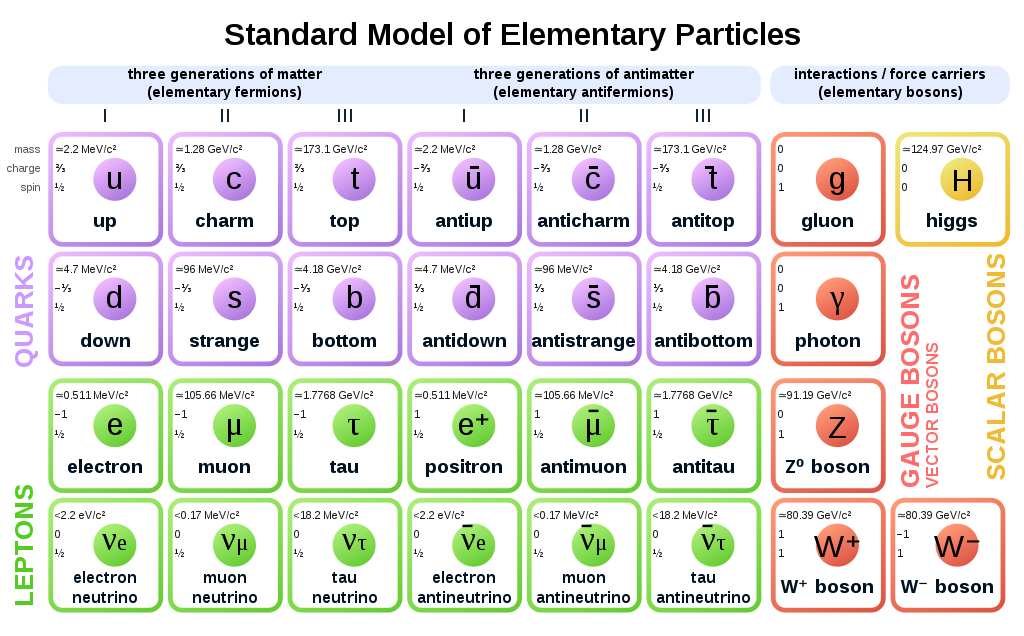
\includegraphics[height=9cm]{1024px-Standard_Model_of_Elementary_Particles_Anti.png}
	\caption{Elementary particles in the Standard Model.\cite{sm_particles}}
	\label{fig:sm-table}
\end{figure}

The SM not only accounts for the matter composition, but also explains the interaction of fermions and bosons in a picture where they interact through exchange of certain force carriers which are bosons as well. More specifically, each set of these carriers mediate one type of fundamental interaction. The force in which most of classical objects interact is electromagnetic interaction and it's mediated by photons. The force that plays a role in the $\beta$ decay is weak interaction, of which the mediators are $\textit{W}$ and $\textit{Z}$ bosons. When a proton and a neutron interact within a nuclei transforming into each other, the actual force carriers are 8 types of gluons (or $\pi$ mesons between nucleus), and it's called strong force. Last but not least, in the quantum field theory, all of these particles has zero mass if there's no spontaneous symmetry breaking by introducing one another boson - Higgs boson, in the Lagrangian formalism of all interactions. With this being said, the ``mass'' is taken as the weight of how strong all these particles interact with Higgs field.

 This complete set of elementary particles describes the whole picture of the Standard Model. It leads to a comprehensive and symmetric theory of fundamentals in particle dynamics. However, the SM prediction does not perfectly match with experimental observations. Since the day theory was built, generations of particle physics experiments have been searching for evidences beyond the SM, as known as New Physics (NP). New Physics is expected to unfold a more profound truth of nature which hopefully explains these observed mismatches. The studies on these fields naturally draw a large attention from modern physicists, focusing on discovering and explaining the mismatches between the SM predictions and experiments. Among these research fields, the studies of symmetry violations (or called as asymmetries) plays an important role. The studies of symmetries was once the driving force for physicists when building the modern theory about particle physics. It is no wonder that now the violation of symmetries, which  physicists didn't expect to happen , has become the cutting edge research topics for New Physics. 





\section{Symmetry Violation}
Symmetries have been one of the focuses in modern physics research since physicists found the internal link between symmetries and conservation laws. The invariance of physical system under infinitesimal transformation is regarded as "continuous symmetry". For instance, any infinitesimal shift on space and time holds physics law in the same form, which implies the physical processes should hold the conservation law of momentum and energy. Such statement is stated as ``Noether’s theorem"\cite{noether}.  Symmetries become a powerful tool in discovering physics laws due to this reason. When the known symmetries are found to be broken, it usually leads to a discovery of the new theory.


There are three types of discrete symmetric operations which play important roles in particle physics. Charge-conjugation $\textit{C}$ is the operation that turns particle to its anti-particle. Parity transformation $\textit{P}$  is the one that puts a negative sign before all the spatial related vector such as $\overrightarrow{r} \to -\overrightarrow{r}$, feeling like look at a physical process in a mirror. The time-reversing operation $\textit{T}$ is to reversely proceed a physical process backward time.  Physicists are convinced that each of these three kinds of symmetric operations makes no change to any physical system. In 1950s, Lee and Yang \cite{PhysRev.104.254} first questioned that parity symmetry might be broken in weak interactions. They offered a few possible ways to test it and then by Wu \cite{Wu_exp}, an observation on the $\beta$ decay of $^{60}$Co was presented that the electrons emitted from  $^{60}$Co decay prefer to flying against the direction of nuclear spin that can be control by the external magnetic field, see Figure \ref{fig:Co60}.

\begin{figure}[htbp]
	\centering
	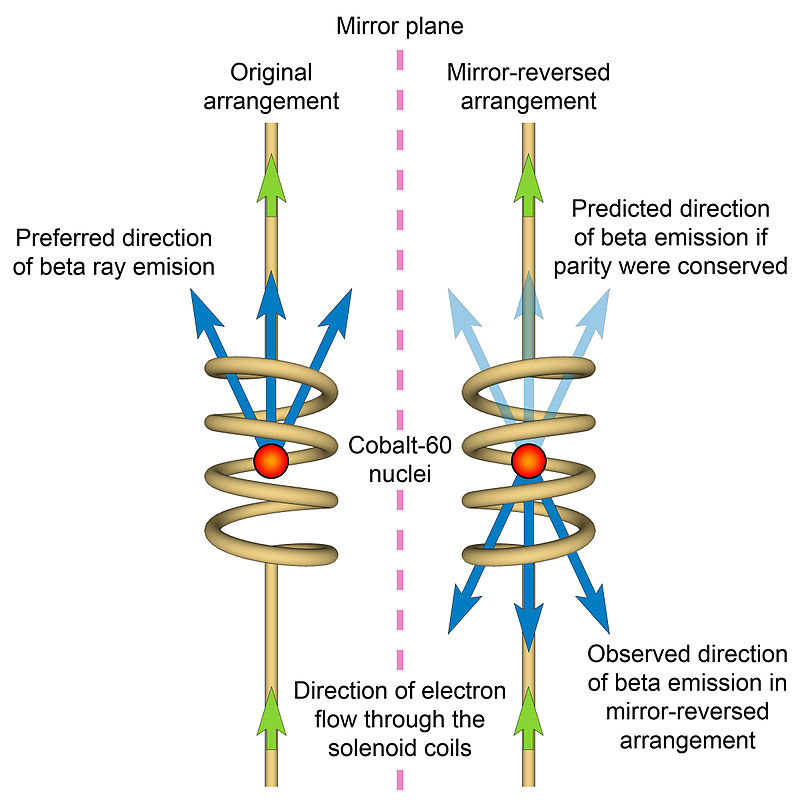
\includegraphics[height=8cm]{DsBxU.jpg}
	\caption{$^{60}$Co decay violates the parity because of the unbalance of electron emissions.}
	\label{fig:Co60}
\end{figure}

Soon, the fact that coupling of weak interaction only involves either neutrinos (left-handed) or anti-neutrinos (right-handed) was realized. So $C$ symmetry is also violated since no left-handed anti-neutrino was found which should be theocratically possible in weak interaction. But if one performs $CP$ operation on such weak interaction involving neutrinos, then such process ``seems" to be equally possible, indicating the conservation of $CP$ in weak interaction for a moment. 

The first evidence of $CP$ violation was found in the Kaon system. Charged Kaon identification was called mystery of ``$\tau - \theta$", because they yield different decay modes with different parity, but have identical mass between $\tau$ and $\theta$. It turns out that they are both charged Kaon meson $K^{+}$, whose decay violates the conservation of $\it{CP}$. In the neutral Kaon system, Cronin and Fitch's experiment was the first experiment that proves the violation of $CP$. They measured the decay products at 57 foot of a neutral kaon beamline assuming all the particle in the beam should be long lifetime $K_L$, nearly no $K_S$. But 0.002\% of them decay through the $K_L \to \pi^+ \pi^-$ ($CP=1$ in final states, yet $K_L$ has  $CP=-1$ ). Given that the expected distance to have 0.002\% of $K_S$ at about speed of light is no more than 1 meter, such deviation at 57 foot is an obvious evidence that $CP$ conservation is also violated in the neutral Kaon system.

In 1973, Kobayashi and Maskawa introduced the third generation of quarks, and the mixing of flavor eigenstates and weak eigenstates is described by a $3\times3$ unitary matrix, which is called Cabibbo-Kobayashi-Maskawa (CKM) matrix\cite{CKM}. The theory allows a free complex phase in CKM matrix and it accounts for the origin of $CP$ asymmetries of weak interactions in the Standard Model. The experimental evidence of $CP$ violation in $b$ meson system was observed in 2001 by Belle and Babar Collaborations. They measured the time-dependent decay time difference of $B$ and $\bar{B}$ in the decay of $B\to J/\psi K_S^0$. This channel provided a outstandingly clearness in theoratical prediction and has relatively large branching fraction, thus it's called the ``golden mode". In 2008, Kobayashi and Maskawa were rewarded the Nobel Prize to highly value their contribution in the discovery of the mechanism of the $CP$ violation. The Belle experiment was regarded as a great success for validating the theory. Later in 2010, the upgrade of Belle, Belle II and the upgrade of KEK accelerator, SuperKEKB, were both approved by Japan to further push the understanding of $CP$ violation in $b$ sector along with other excitingly interesting topics in New Phsyics. 

\section{CKM mechanism}
\begin{comment}
Three kinds of fundamental interaction: weak, strong and electromagnetic interactions have been included in the SM. The SM can inherently solve the origin of the symmetries and asymmetries, with the theoretical support from quantum field theory (QFT). In QFT, the particles are treated as the excitation of its field and the interaction between particles can also be treated as the exchange of energy and momentum between particles. Enlighten by many aspects in classical mechanism, QFT is also built on a formalism in which the Lagrangian plays an essential role. The difference is field, as a physical entity, is universally distributed in space-time, whereas classical objects can only exist with a local position. Given this fact, it is natural to define the Lagrangian of field as a ``density" of Lagrangian of particles. In the SM, for instance, a fermion field $\it{\Psi}$ with mass $m$ is described by a field as follows:

\begin{equation}
\mathcal{L}_0 = \it{\overline{\Psi}(i\gamma^\mu \partial_\mu-m)\Psi}
\end{equation}

Such form presents a field which will fit in Lorentz transition and space-time transition. Then gauge theory is used to describe the interaction of fermions so that the Lagrangian should be invariant under the local gauge transformation. There are different types of local gauge transformations, as well as their invariance. 
Group is the mathematical term used to describe transformation invariance. Each group has a basic presentation of matrix. If every elements in a group can find a corresponding matrix which keeps their relations in multiplying operation,then the smallest dimension of such matrix is called basic matrix presentation. If the matrix elements are Unitary, n dimension, such group is called$\it{U}$(n), 
specially if the anti-matrix is the conjugation-transverse of itself, such group is called Special Unitary.($\it{SU}$(n)) 


For instance, in the U(1) gauge transition, if one requires the invariance of electromagnetism by adding $\it{U}$(1) gauge, the Maxwell formalism naturally fits in the quantum electroweak dynamics (QED), along with the weak interaction which is invariant under not only $\it{U}$(1) transformation but also $\it{SU}$(2). The symmetry of electromagnetic force and weak force is spontaneously broken due to the non-zero expected value of Higgs field of the vacuum. That makes the coupling of different field varied so the carriers of electromagnetic field and weak field diverged. Massless particle $\gamma$ is carrying the electromagnetic force. $W^{+/-}$ and neutral $Z$ deliver the force of weak interaction. They have different coupling strength to the Higgs field, which excites a neutral particle, Higgs boson $H$. The quarks, however, not only coupling to $W^{+/-},Z$ by weak interaction, they directly interact with each other by exchanging gluons by strong force. The strong interaction is described by $SU$(3) with eight types of different gluons, and every gluon has 3 colors. The mechanism that describes this interaction is called ``quantum chromodynamics" (QCD). 

The contribution of the origin of $CP$ violation is mainly from the weak current in the SM Lagrangian. So the discussion of the theoretical interface of $CP$ violation will be focusing on the weak interaction. In the Lagrangian formalism in the SM, gauge interactions are described by the terms in the Lagrangian in a form that quark field is coupling with each other through gauge current, specifically the weak or neutral current. In order to keep the $SU$(2) symmetry treating the quarks from same generation equally, the weak eigenstates are introduced for presenting the Lagrangian. However, if we require the gauge bosons $W^{+/-}$ and $Z$ acquire mass from Yukawa coupling with Higgs field, the term that describes the weak interaction is spontaneously breaking under $CP$ operation. 

\end{comment}


 


\begin{equation}{\label{Eqn:higgs_field}}
\large
\Phi = 
\begin{pmatrix}
\phi^+\\
\nu + \frac{H+i\chi}{\sqrt{2}}
\end{pmatrix}
\end{equation}

 Equation \ref{Eqn:higgs_field} is the Higgs potential doublets. $H$'s value is 174 GeV as the expected Higgs potential for vacuum and $\phi$ and $\chi$ are the pseduo-Goldstone fields which are appearing when introducing Higgs field  $\phi$ without breaking the gauge symmetry. The idea of introducing Higgs is to naturally solve the mass origin of particles under the gauge symmetry in the SM, as Equation  \ref{yukawa_coupling} presents. 

\begin{equation}{\label{yukawa_coupling}}
\large
\mathcal{L}_{Yuk}^q = 
-{Q}^\dag Y^d \Phi d_R^\prime 
-{Q}^\dag Y^u \epsilon \Phi^* u_R^\prime
+ h.c.
\end{equation}

Here the primed fields stand for the weak eigenstates of quarks. $\epsilon$ is a 2$\times$ 2 matrix. $Q^\dag$ is the left-handed doublets that stand for weak eigenstates of up and down types quarks. 

\begin{equation}
\large
\epsilon =  
\begin{pmatrix}
0 & 1\\
-1 & 0
\end{pmatrix}
\end{equation}

\begin{equation}
\large
Q =  
\begin{pmatrix}
u^\prime & d^\prime \\
c^\prime & s^\prime \\
t^\prime & b^\prime
\end{pmatrix}_L
\end{equation}
Yukawa matrix is an arbitrary 3 $\times$ 3 complex matrix $Y^{u,d}$ which give the rise of two types of massive quark field $M^{u,d}=Y^{u,d}\nu$. The choosing the weak eigenstates makes these matrices un-diagnosed. So the ``rotation" of weak eigenstates to diagnose them is done by:

\begin{equation}\label{rot1}
\small
S_{L,R}^{u}
\begin{pmatrix}
u^\prime   \\
c^\prime  \\
t^\prime 
\end{pmatrix}_{L,R}
= \begin{pmatrix}
u  \\
c  \\
t 
\end{pmatrix}_{L,R}
\end{equation}

\begin{equation}\label{rot2}
\small
S_{L,R}^{d}
\begin{pmatrix}
d^\prime   \\
s^\prime  \\
b^\prime 
\end{pmatrix}_{L,R}
= \begin{pmatrix}
d  \\
s  \\
b 
\end{pmatrix}_{L,R}
\end{equation}


 In Equation \ref{rot1} and \ref{rot2}, $S^{u,d}_{L,R}$ are all unitary matrices since they are actually generated by the normalized eigenstate vectors of the Yukawa matrix, which means ${S_{L,R}^{u,d}}^\dag S_{L,R}^{u,d} = I$. The mass
  items $M_q$, arised after the ``rotation" can be presented as: 
\begin{equation}
\mathcal{L}_{m} = -\sum_{q=u,c,t,d,s,b}^{} M_q q^{\dag}_{} q_{}
\end{equation}
where $q=(q_L+q_R)$ is four-component Dirac field, and $q_L^\dag q_L = q_R^\dag q_R = 0$. The matrix $S^{u,d}_{L,R}$ are contributing to the weak interactions as Equation \ref{weak_coupling} shows.
\begin{equation}\label{weak_coupling}
\small
\mathcal{L}^q_W = \frac{g}{\sqrt{2}}
\begin{bmatrix}
\begin{pmatrix}
\overline{u}&\overline{c}&\overline{t}
\end{pmatrix}_L

\gamma^\mu W^{+}_{\mu}
%{S^{u}_{L}}^{\dag}
%S^{d}_{L}
V_{CKM}
\begin{pmatrix}
d\\s\\b\\
\end{pmatrix}_L+
\begin{pmatrix}
\overline{d}&\overline{s}&\overline{b}
\end{pmatrix}_L
\gamma^\mu W^{-}_{\mu}
%S^{u}_{L}
%{S^{d}_{L}}^{\dag}
V_{CKM}^{\dag}
\begin{pmatrix}
u\\c\\t\\
\end{pmatrix}_L
\end{bmatrix}
\end{equation}

%\begin{equation}
%V_{CKM} = 
%{S^{u}_{L}}^{\dag}
%S^{d}_{L}
%\end{equation}
The Lagrangian hereby clearly declair the transition of different charged quarks through the coupling of charged current $W^{+/-}$. Interestingly, such coupling only applies for the left-handed quarks. For example, a left-handed c quark only transits to left-handed s quark by giving out a $W$ boson. If the Parity conjugation is applied to the Lagrangian, the left-handed quarks becomes right-handed. The same thing happens if the Charge conjugation is applied, cause it changes the chirality of the 4 components quark fields and charge sign at the same time. This means the weak interaction will not conserve the Parity and the Charge symmetries. However, if the $CP$ conjugation is applied, all left-handed quark fields' chirality are  unchanged and only the conjugation of quark fields are made, as Equation \ref{cp-conj} shows.
\begin{equation}\label{cp-conj}
\small
\large
\begin{pmatrix}
\overline{u}&\overline{c}&\overline{t}
\end{pmatrix}_L
\gamma^\mu W^{+}_{\mu}
V_{CKM}
\begin{pmatrix}
d\\s\\b\\
\end{pmatrix}_L
{\Leftrightarrow}
\begin{pmatrix}
{u}&{c}&{t}
\end{pmatrix}_L
\gamma^\mu W^{-}_{\mu}
{V_{CKM}}
\begin{pmatrix}
\overline d\\\overline s\\\overline b\\
\end{pmatrix}_L
\end{equation} 

Comparing  Equation \ref{cp-conj} and \ref{weak_coupling}, the $\it{CP}$ symmetry requires: 

\begin{equation}\label{cp_cons}
\large
{u_{L}^i}V_{ij} \bar{d}^{j}_L \gamma^\mu W^{-}_{\mu}
=
{{u}^{n}_LV^{*}_{nm}\bar{d}_{L}^m}  \gamma^\mu W^{-}_{\mu}
\end{equation}
The same indices $ij$ and $nm$ are summed over on both side. This is equivalent to: 
\begin{equation}\label{v-eq}
V_{ij} = V^{*}_{ij}
\end{equation}
On the one hand, if the CKM matrix is real, $CP$ will be conserved in the weak interaction in the SM. On the other hand, from Equation \ref{cp_cons}, it's still possible to make Lagrangian unchanged even if $V_{CKM}$ is not real. By introducing non-physical phases for each quark field $u^k_L e^{(i\phi_{uk})}$ and $d^j_L e^{(i\phi_{dj})}$, the Equation \ref{v-eq} becomes:
\begin{equation}
\Large
V_{kj} e^{i(\phi_{dj}-\phi_{uk})} = V^{*}_{kj}e^{i(\phi_{uk}-\phi_{dj})}
\end{equation}

Assuming the complex phase of CKM $kj$-th element is $\theta_{kj}$, it's obviously required that:
\begin{equation}
\large
\theta_{kj} = \phi_{uk}-\phi_{dj}
\end{equation}
 Historically, before the 3rd generation of quarks is discovered, $k,j$ can only be either 1 or 2, and $V_{CKM}$ is 2 dimensional unitary matrix. With two generations of quarks, there are 8 real parameters in CKM matrix, 4 describe amplitudes and 4 describe complex phases. Unitary condition $V_{CKM}{\dag} V_{CKM} = 1$ gives 4 equations, containing 2 real equations and 2 complex equations. The 2 complex equations are identical so only 3 independent equations arise.
2 complex equations leads to 2 equations about phases plus 2 equations are about amplitude. Based on this, the degree of freedom of phases on 2 dimensional CKM matrix is $4-2=2$. Thus it's always possible to make CKM real by properly render the non-physical phases.
This means with only existence of 2 generations of quarks, there is no spontaneous explanation for $CP$ violation in the SM. When Kobayashi and Maskawa realized that this is no longer true if 3rd generation of quarks exists, they presented CKM matrix as a 3 $\times$ 3 matrix. In such case, there will always be one irreducible complex phase parameter in the CKM matrix, which means $\it{CP}$ symmetry is no longer conserved in the weak interactions. 
\begin{comment}
Assuming the free phases are $\theta_{11}$ and $\theta_{22}$.Eq(2.15) presents: 
\begin{equation}
\large
\begin{pmatrix}
\theta_{11}\\
\theta_{22}
\end{pmatrix}
=
\begin{pmatrix}
1&-1&0&0\\
0&0&1&-1
\end{pmatrix}
\begin{pmatrix}
\phi_{u1} \\
\phi_{d1} \\
\phi_{u2} \\
\phi_{d2}
\end{pmatrix}
\end{equation}.
which is always render-able by properly choosing non-physical phases. 
\end{comment}




\begin{comment}
 As a result, Eq(1.15) is equivalent to (the order of complex phases is arbitrary since only the degree of freedom matters at last ): 

\begin{equation}
\large
\begin{pmatrix}
\theta_{11}\\
\theta_{22}\\
\theta_{33}\\
\theta_{12}\\
\theta_{23}\\
\theta_{13}
\end{pmatrix}
=
\begin{pmatrix}
1&-1&0&0&0&0\\
0&0&1&-1&0&0\\
0&0&0&0&1&-1\\
1&0&0&-1&0&0\\
0&0&1&0&0&-1\\
1&0&0&0&0&-1
\end{pmatrix}
\begin{pmatrix}
\phi_{u1} \\
\phi_{d1} \\
\phi_{u2} \\
\phi_{d2} \\
\phi_{u3} \\
\phi_{d3} 
\end{pmatrix}
\end{equation}
if we choose the up-right half of phases as free ones. It's easily to see that 5 phases can be canceled by non-physical 6 phases but since the rank of the 6 $\times$ 6 co-efficient matrix in Eq(1.16) is 5, there's still one physical phase as the parameter that gives rise to $CP$ violation exists, named as $\delta_{KM}$. This accounts for the $\it{CP}$ violation through exchange of charged currents.

Similar to the Eq(1.11), the flavor changing neutral current transit quarks among the same sides, called FCNC process. Such transition renders the coupling of neutral gauge bosons with quarks, for example,through $Z$ boson,  the neutral current coupling is:

\begin{equation}
\large
\begin{split}
\mathcal{L}^q_Z & = \frac{g}{\sqrt{2}}
\begin{bmatrix}
\begin{pmatrix}
\overline{d}&\overline{s}&\overline{b}
\end{pmatrix}_L
\gamma^\mu Z^{0}_{\mu}
{S^{d}_{L}}^{\dag}
S^{d}_{L}
\begin{pmatrix}
d\\s\\b\\
\end{pmatrix}_L+
\begin{pmatrix}
\overline{u}&\overline{c}&\overline{t}
\end{pmatrix}_L
\gamma^\mu Z^{0}_{\mu}
S^{u}_{L}
{S^{u}_{L}}^{\dag}
\begin{pmatrix}
u\\c\\t\\
\end{pmatrix}_L
\end{bmatrix} \\
& = \sum_{q=u,c,t,d,s,b}^{}  Z^{0}_{\mu}\bar{q_L} \gamma^\mu q_L
\end{split}
\end{equation}
Noted that here $S^{u,d}_{L,R}$ is unitary. And there is no crossing term means that with the tree level gauge interaction, FCNC processes are largely forbidden. This mechanism is called GIM mechanism, which only allows the gauge interaction coupling to same side quarks in neutral current so the $SU$(2) symmetry is conserved. But connecting two tree level vertices, a quark can transit to same charged quarks by a loop diagram. Two typical types of such processes are box diagram and penguin-mode diagram. 

\begin{figure}[H]
	\begin{minipage}[t]{0.5\linewidth} % 如果一行放2个图,用0.5,如果3个图,用0.33
		\centering 
		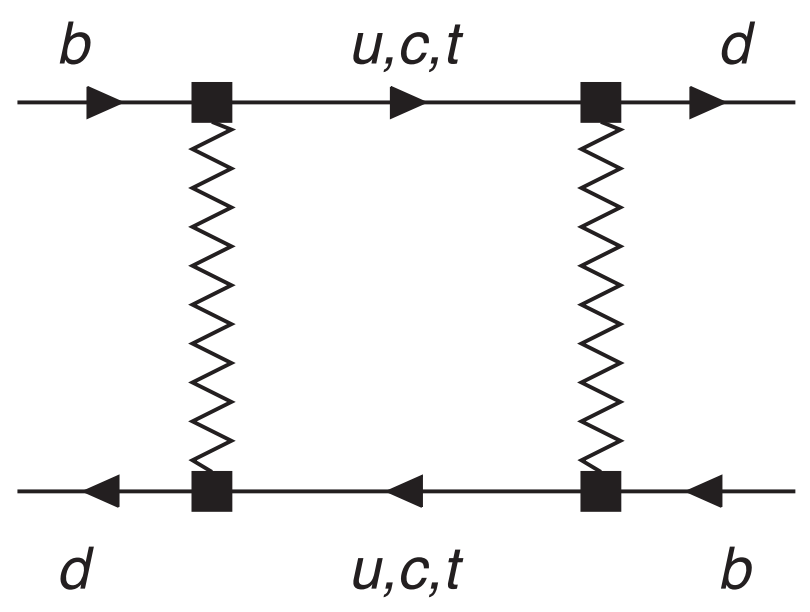
\includegraphics[width=2in]{BBbox} 
		\caption{Box diagram for $B^0$ meson} 
		\label{fig:side:a} 
	\end{minipage}% 
	\begin{minipage}[t]{0.5\linewidth} 
		\centering 
		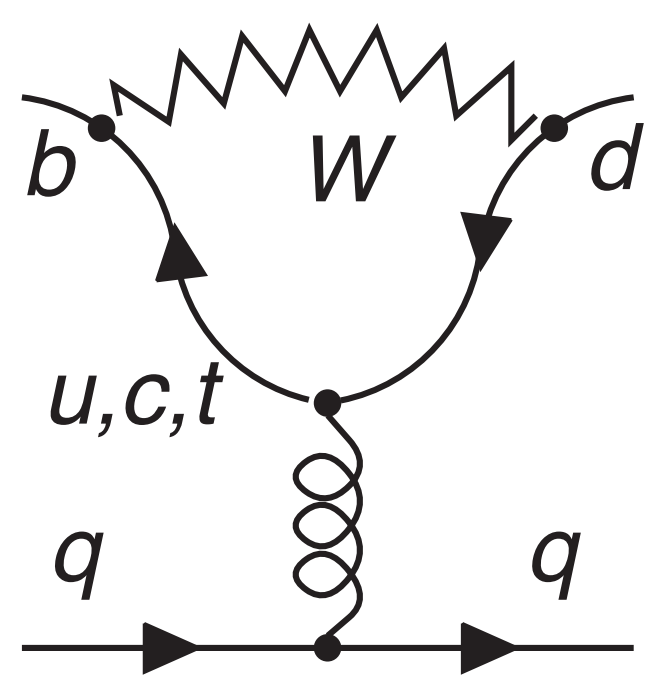
\includegraphics[width=1.5in]{penguin} 
		\caption{penguin mode diagram} 
		\label{fig:side:b} 
	\end{minipage} 
\end{figure}
In Fig(1-3), the amplitude of such process depends on the mass of $W^{+/-}$ boson and  virtual intermediate quarks, in a form of:
\begin{equation}
\Large
\mathcal{A}=
\sum_{q=u,c,t}^{}
V_{qb}^{*}V_{qd} f
\begin{pmatrix}
\frac{m^2_q}{m^2_W}
\end{pmatrix}
\end{equation}
Using the unitary condition of CKM matrices,it becomes: 
\begin{equation}
\Large
\mathcal{A}=
V^*_{tb}V_{td}
\begin{bmatrix}
\frac{f}{M_W^2}
(m^2_t-m^2_c)
\end{bmatrix}
+
V^*_{ub}V_{ud}
\begin{bmatrix}
\frac{f}{M_W^2}
(m^2_u-m^2_c)
\end{bmatrix}
\end{equation}
Unexpected large mixing of $B^0_d-\bar{B^0_d}$ is hinting that the top quark could be much heavier since the up and charm quark mass difference is much smaller than the mass of $W$ boson. The amplitude in Eq(1.19) is dominant by first term, namely by the mass of top quark. 

By the discussion above, FCNC processes are largely suppressed in the SM but sensitive to the  New Physics because the unexpected amplitudes could be hints for new coupling forbidden in the SM or even the new intermediate states. The measurement of CKM  properties are the focus to validates the Yukawa sector of the SM and any large deviation could kick the door to New Physics.  
\end{comment}
%\section{Unitary Angles of CKM}
The $3\times 3$ unitary CKM matrix can be written as Equation \ref{CKM}.
\begin{equation}\label{CKM}
\large
V_{CKM}=
\begin{pmatrix}
V_{ud} & V_{us} & V_{ub}\\
V_{cd} & V_{cs} & V_{cb}\\
V_{td} & V_{ts} & V_{tb}\\
\end{pmatrix}
\end{equation}

It can be parameterized:
\begin{equation}
V_{CKM}=
\begin{pmatrix}
c_{12}c_{13} & s_{12}c_{13} & s_{13}e^{-i\delta }\\
-s_{12}c_{23}-c_{12}s_{23}s_{13}e^{-i\delta } &c_{12}c_{23}-s_{12}s_{23}s_{13}e^{-i\delta } & s_{23}c_{13}\\
s_{12}s_{23}-c_{12}s_{23}s_{13}e^{-i\delta }  & -c_{12}c_{23}-s_{12}c_{23}s_{13}e^{-i\delta } & c_{23}c_{13}
\end{pmatrix}
\end{equation}
where the $c_{jk}=\text{cos}(\theta_{jk})$ and $s_{jk}=\text{sin}(\theta_{jk})$, $\delta$ is the irreducible complex phase. By measuring the relative branching ratio of $b\to c$, $s\to u$ and $b\to u$ in a tree level transitions: 
\begin{equation}
|V_{ub}|\ll |V_{cb}|\ll |V_{us}|
\end{equation}

and the following relations are often used to simplify CKM matrix presentation:
\begin{equation}\label{ckm_par1}
s_{13}=\lambda , s_{23}=A\lambda^2, s_{13}e^{i\delta}=A\lambda^3(\rho-i\eta)
\end{equation}
% 2021.01.23 ends 
By using Equation \ref{ckm_par1}, CKM matrix is parameterized as:
\begin{equation}
V_{CKM}=
\begin{pmatrix}
1-1/2\lambda^2 & \lambda & A\lambda^3(\rho-i\eta)\\
-\lambda & 1-1/2\lambda^2 & A\lambda^2\\
A\lambda^3(\rho-i\eta) & -A\lambda^2 & 1
\end{pmatrix}+\mathcal{O}(\lambda^4)
\end{equation}

Using the unitary condition, the following equation is obtained.
\begin{equation}\label{ckm_triangles}
1+
\frac{V_{ud}V^*_{ub}}{V_{cd}V^*_{cb}}+
\frac{V_{td}V^*_{tb}}{V_{cd}V^*_{cb}}
=0
\end{equation}
Plotting the relation in a complex 2D plane using Equation \ref{ckm_triangles},
\begin{figure}[htpb]
	\centering
	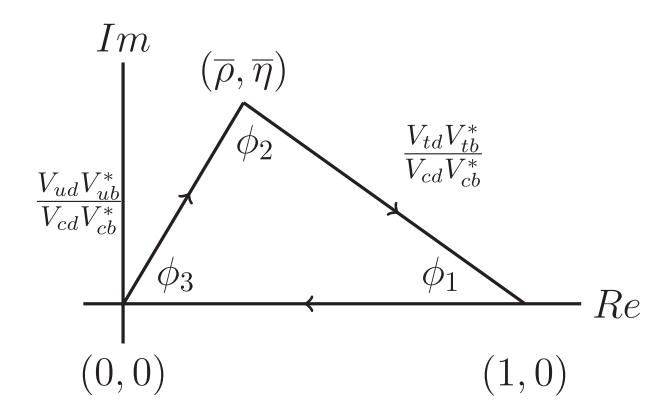
\includegraphics[height=6cm]{UT}
	\caption{The unitary angles of CKM}
	\label{fig:ckm_angles}
\end{figure}
\begin{eqnarray}
\bar{\rho}+i\bar{\eta}=- \frac{V_{ud}V^*_{ub}}{V_{cd}V^*_{cb}}\\
1-(\bar{\rho}+i\bar{\eta})=-\frac{V_{td}V^*_{tb}}{V_{cd}V^*_{cb}}
\end{eqnarray}
These angles are obtained by drawing the $(\bar{\rho},\bar{\eta})$ on the complex coordinates, and they are also well-known in the names as: $\phi_1=\beta,\phi_2=\alpha,\phi_3=\gamma$. The results presenting the measurement of CKM angles or $(\bar{\rho},\bar{\eta})$ in 2019 is shown in Figure \ref{fig:ckm19}.
\begin{figure}[htbp]
	\centering
	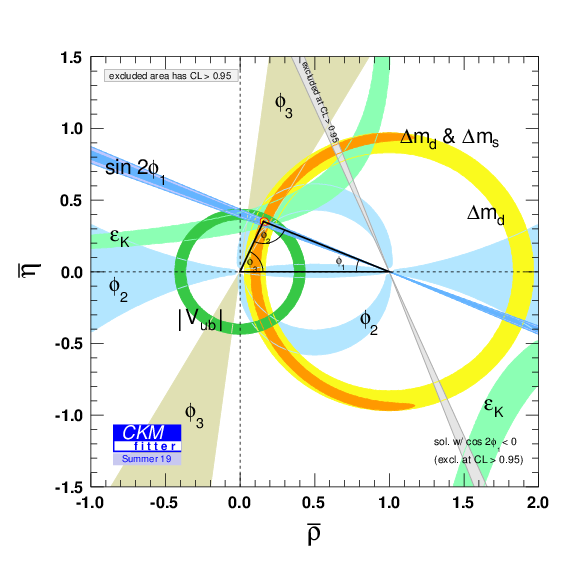
\includegraphics[height=8cm]{ckm19}
	\caption{The CKM angles fit in the complex plane of $\bar{\rho}-\bar{\eta}$.\cite{ckmfitter}}
	\label{fig:ckm19}
\end{figure}

The measurement of $\phi_1$ and $\phi_2$ are coming from the time-dependent $CP$ violations (TDCPV). $\phi_1$ in the tree-level dominated decays has been precisely measured thanks to the small hadronic uncertainties. FCNC process rises through the $B^0_d-\bar{B^0_d}$ mixing in box diagram, and it's believed that potential New Physics processes might contribute to the difference in between results of CKM angles measured from experiments. For example, angle $\phi_1$ that is observed from tree-level dominated process like $B^0 \to J/\psi K^0_s$ could be different from penguin-dominated $b \to s$ transition. The Standard Model provides an approximated correction on how large the deviation might be, where it requires much precise measurement on each decay channel to validate the potential New Physics effect. The prospective large Belle II data and more precise time resolution performance will be much helpful to clear the tension in future. 

\section{Time Dependent $CP$ violation}
\subsection{ $CP$ violation in neutral B system}
The  $\phi_1$,$\phi_2$ and $\phi_3$ are essentially measuring the CKM $CP$ violating phase since there's only one complex phase in CKM and it can be determined by these 3 angles. And $\phi_{1,2}$ are related to mostly in the time dependent decay rate difference. From Figure \ref{fig:ckm_angles}, one can obtain: 
\begin{eqnarray}
\phi_1=Arg(-\frac{V_{td}V^*_{tb}}{V_{cd}V^*_{cb}})\\
\phi_2=Arg(-\frac{V_{td}V^*_{tb}}{V_{ud}V^*_{ub}})
\end{eqnarray}

The general strategy to extract the $\phi_{1,2}$ is to measure the time-dependent $CP$ violation.
The mass eigenstates which are driving the propagation of B meson states in the mixing are: $|B\rangle_{H,L}=p|B\rangle \pm q|\overline{B}\rangle $, where $H$ and $L$ stand for the larger and smaller eigenvalues corresponded states. $|B\rangle$ and $|\overline{B}\rangle$ are the flavor eigenstates.
The Hamiltonian matrix can be written using flavor eigenstates: 
\begin{equation}
M_\Gamma=
\begin{bmatrix}
m-i/2\Gamma & M_{12}-i/2\Gamma_{12}\\
M^*_{12}-i/2\Gamma^*_{12}& m-i/2\Gamma 
\end{bmatrix}
\end{equation}

and the time evolution of mass eigenstates are defined as (using the notation of $B_{H,L}$ as physical states at $t = 0$): 
\begin{eqnarray}
B_H(t)=e^{-im_Ht}e^{-\Gamma_Ht/2}B_H\\
B_L(t)=e^{-im_Lt}e^{-\Gamma_Lt/2}B_L
\end{eqnarray}
where $M_{H,L}$ and $\Gamma_{H,L}$ are the masses and decay width of two mass eigenstates. By expanding the mass eigenstates using flavor eigenstates, 
\begin{eqnarray}
B(t)=(1/2p)e^{-im_Ht}e^{-\Gamma_Ht/2}(pB+q\bar{B})+(1/2p)e^{-im_Lt}e^{-\Gamma_Lt/2}(pB-q\bar{B})\\
\bar{B}(t)=(1/2q)e^{-im_Ht}e^{-\Gamma_Ht/2}(pB+q\bar{B})-(1/2q)e^{-im_Lt}e^{-\Gamma_Lt/2}(pB-q\bar{B})
\end{eqnarray}
and replacing $g_{\pm}(t)=\frac{1}{2}(e^{-im_Ht-\Gamma_H/2t}\pm e^{-im_Lt-\Gamma_L/2t})$, above two equations become:
\begin{eqnarray}
B(t)=g_{+}(t)B +\frac{q}{p}g_{-}(t)\bar{B}\\
\bar{B}(t)=g_{+}(t)\bar{B} + \frac{p}{q}g_{-}(t){B}
\end{eqnarray}
Considering all the phases space of the decay from flavor eigenstates to final states $f(\bar{f})$ are included in the amplitudes $\mathcal{A}_f (\bar{\mathcal{A}}_f)$, one needs to expand the flavor eigenstates using such amplitude to have the differential decay rate $\Gamma(B\to f,t)$. From $B(t) \propto \mathcal{A}_f\psi_f+h.c $ and $ (\bar{B}(t) \propto \bar{\mathcal{A}_f}\psi_{\bar{f}}+h.c)$:
\begin{eqnarray}
\Gamma(B\to f,t)=|\mathcal{A}_f|(|g_+(t)|^2+|\lambda_f|^2|g_-(t)|^2+2Re(\lambda_f g^*_+(t)g_-(t))),\\
\Gamma(\bar{B}\to \bar{f},t)=|\bar{\mathcal{A}_{\bar{f}}}|(|g_+(t)|^2+|\bar{\lambda}_{\bar{f}}|^2|g_-(t)|^2+2Re(\bar{\lambda}_{\bar{f}} g^*_+(t)g_-(t)))
\end{eqnarray} where the parameter $\lambda_f$ is
\begin{eqnarray}
\lambda_f \equiv (q/p) (\bar{\mathcal{A}}_f / \mathcal{A}_f)\\
\bar{\lambda}_{\bar{f}} \equiv (q/p) ( \mathcal{A}_{\bar{f}}/\bar{\mathcal{A}}_{\bar{f})}
\end{eqnarray} 
$q/p$ is introduced by the coefficient of mass eigenstates from weak eigenstates. Using the Hamiltonian matrix, $q/p$ can be presented as: 
\begin{equation}
	q/p = \frac{\Delta M - i/2 \Delta \Gamma}{2(M_{12}- i/2 \Gamma_{12})}
\end{equation}
where the $M_{12}$ and $\Gamma_{12}$ stands for the contribution of non-diagnosed term in the Hamiltonian matirx. $\Delta{M}=M_H-M_L$ and $\Delta{\Gamma}=\Gamma_H-\Gamma_L$ are the difference of mass and decay width for two mass eigenstates.
It's obvious that if $|A_f| \neq |\bar{A}_{\bar{f}}|$, direct $\it{CP}$ violation will occur.  

The time-dependent decay rate difference is defined as Equation \ref{Acp}:
\begin{equation}\label{Acp}
\begin{split}
A_{CP}(t)&\equiv \frac{\Gamma(B\to f,t)-\Gamma(\bar{B}\to \bar{f},t)}{\Gamma(B\to f,t)+\Gamma(\bar{B}\to \bar{f},t)}\\
&=\frac{S_f sin(\Delta{M}t)-A_fcos(\Delta{M}t)}
{cosh(\Delta \Gamma t/2)+A^f_{\Delta \Gamma}sinh(\Delta \Gamma t/2)}
\end{split}
\end{equation},where
\begin{equation}\label{cp-parameters}
\mathcal{S}=\frac{2Im(\lambda_f)}{1+|\lambda_f|^2};\mathcal{A}=\frac{1-|\lambda_f|^2}{1+|\lambda_f|^2};A^f_{\Delta \Gamma}=-\frac{2Re(\lambda_f)}{1+|\lambda_f|^2}
\end{equation}
%and noted with A
%\begin{eqnarray}
%|g_{\pm}(t)|^2=\frac{e^{-\Gamma t}}{2}(cosh(\frac{\Delta \Gamma t}{2})\pm cos(\Delta m t))\\
%g_{+}^*(t)g_{-}(t)=\frac{e^{-\Gamma t}}{2}(sinh(\frac{\Delta \Gamma t}{2})+ isinh(\Delta m t))
%\end{eqnarray}

 The origin of time is set to the flavor tagged moment.
 %The $\Delta M$ and $\Delta \Gamma$ in $B_d^0-\bar{B_d^0}$ system can be approximately treated as zero. 
 The time-dependent CP violation parameters are $\mathcal{S}$ and $\mathcal{A}$, which are determined by $\lambda_f$.



\subsection{$\phi_1$  from $B^0 \to J/\psi K^0_S$}
If final states are $CP$ definite, the amplitude then equals to: $\mathcal{A}_f \equiv \langle f|H|B\rangle$ and $\bar{\mathcal{A}_f} \equiv \langle f|H|\bar{B}\rangle$. In $B_d^0-\bar{B_d^0}$, $q/p$ can be treated as $e^{i\phi_d}$ safely as pure phase term. This relative phase accounts the transition from $b$ to up-type quarks to $s$ in mixing, so it can be presented as $\phi_d = \text{Arg}(V^*_{td}V_{tb})/(V^*_{tb}V_{td}) \approx 2\phi_1 $ based on negligible correction to the SM. In the golden mode $B^0 \to J/\psi K^0_S$, considering $\Delta \Gamma$ can be treated as zero safely in the Standard Model\cite{dighe2001width} in this case, Equation \ref{Acp} can be reduced to:

\begin{equation}
	A_{CP}(t)=\mathcal{S} \text{sin}(\Delta{M}t)- \mathcal{A}\text{cos}(\Delta{M}t)
\end{equation}

\begin{comment}
Usually, $S_f$ provides a good sensitivity to $\phi_1$ in Eq(1.42) by replacing $\phi_d$ inside $\lambda_f$ since the rest two equations canceled out the complex phase of $(q/p)$. For instance, in the process of  $b\to \bar{c}cs$ ,the amplitude contributions from tree level and loop level diagram can be written in a form as follows using the CKM unitary condition: 
\end{comment}
For decay amplitude, which recieve contribution from tree-level and loop-level processes shown in Figure \ref{fig:jpsiks} , 

\begin{figure}[htpb]
	\centering
	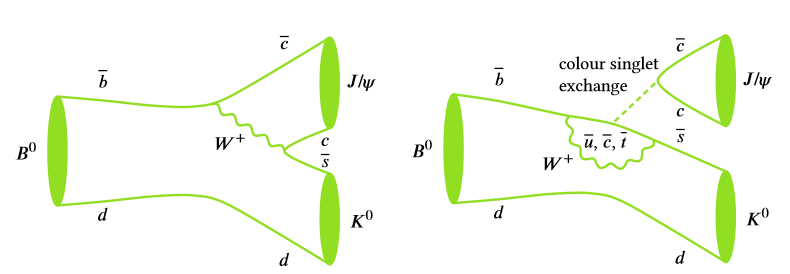
\includegraphics[height=4cm]{jpsiks-diagram}
	\caption{The dominated tree-level (left) and the suppressed loop-level (right) of $B\to J/\psi K^0$, in which $K^0$ particles are detected $K_S^0$. \cite{wishahi2014measurement}}
	\label{fig:jpsiks}
\end{figure}

%\begin{equation}
%	\mathcal{A}_f= 
%	\lambda^s_c T_f + 
%	\lambda^s_u P_f; \\
%	\lambda^q_i = V^*_{ib}V_{iq}
%\end{equation}
%where $T_f$ and $P_f$ stands for leading order contribution of tree and penguin diagrams, see Fig(1-7). Here, the leading term can be presented as: 

Using the relation $|V_{ub}|\ll |V_{cb}|\ll|V_{us}|<|V_{cs}|$, it's obvious that $V^*_{ub}V_{us} \ll V^*_{cb}V_{cs}$, so the penguin-mode is surppressed in the Standard Model. Defining $\eta_f$ as the $\it{CP}$ eigenvalue for $\it{CP}$ definite final states, 
% $\bar{\mathcal{A}}_f / \mathcal{A}_f \approx \eta_f {\lambda^{s}_c}^*/\lambda^{s}_c$, where 


Given $\eta_f=1$ and $|\lambda_f|=1$ in $B^0 \to J/\psi K^0_S$, from \ref{cp-parameters}, $\it{CP}$ parameters can be presented as: 
\begin{equation}\label{SA}
\mathcal{S} = Im(\lambda_f)
=-sin(\phi_d)\eta_f=-sin(2\phi_1) ; \: \mathcal{A} = 0
\end{equation}

From Equation \ref{SA} , $\phi_1$ can be accessed pretty precisely in the measurement of time-dependent $\it{CP}$ violation in $B^0 \to J/\psi K^0_S$, whose branching fraction is relatively high. 
\begin{comment}
In the $b\to q\bar{q}s$ process where flavor $q$ is not charm, similar to the discussion above, we can extract $\phi_1$ using the same method. Moreover, it provides a penguin-dominated process which is sensitive to the contribution of New Physics, which includes the $B^0_d\to K^0_S K^0_S K^0_S$ decay. In the next section, it's clear that such decay process is important to provide additional insight in seeking the effect beyond the SM (BSM contribution).
\end{comment}



\subsection{$\phi_1$ from penguin-dominated mode $b\to q\bar{q}s$}
Compared to $B^0 \to J/\psi K^0_S$ channel, the measurement of $\mathcal{S}$ and $\mathcal{A}$ from penguin-dominated channels through $b \to q\bar{q}s$ where $q$ is $u,d,s$ can be different due to the varied tree-to-penguin amplitude ratio. Furthermore, they are quite interesting for the following reasons\cite{b2book}. First, they can probe $B^0-\bar{B}^0$ through different short-distance vertices than the tree-level dominated decays. Second, the relatively small penguin amplitude may be more sensitive to the NP effects than tree-dominated modes. Last but not least, they comprise a large number of different final states, which can help disentangling non-perturbation long-distance physics from short-distance information, such as $\phi_1$ or NP contributions to the weak Hamiltonian. 

\begin{comment}
First,  the $b\to q\bar{q}s$  gives a different vertex in gluonic decay than tree diagram. 
Second, such process is tree level suppressed but penguin-dominated, so the New Physics effects can be easier to be spotted. The SM agrees with tree level process in percent accuracy so the sub-percent BSM effects may be hard to see. Similar to Fig(1-7), due to FCNC tree level forbidden, 
\begin{figure}[H]
\centering
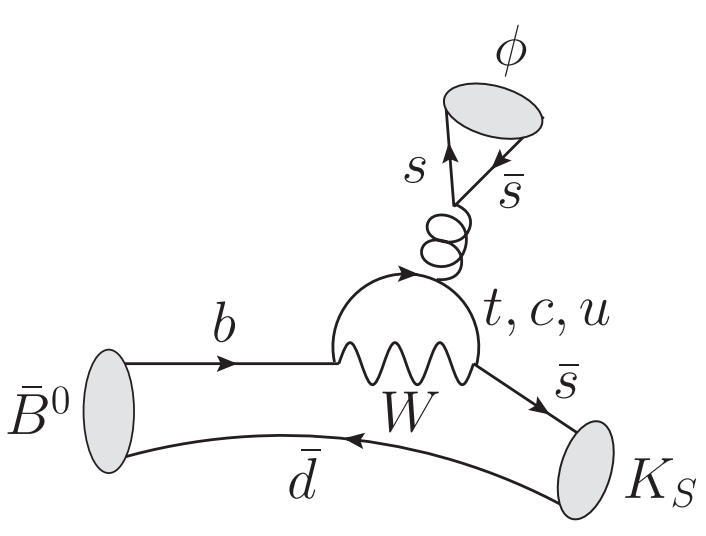
\includegraphics[height=5cm]{Bto3Ks}
\caption{penguin mode $b\to q\bar{q}s$ where $\phi$ is formed by two strange quark as the intermediate state.}
\end{figure}

\end{comment}
Considering possible New Physics contribution as $A_f^{NP}$, the decay amplitude can be rendered as: 
\begin{equation}
\mathcal{A}_f= 
\lambda^s_u T_f + 
\lambda^s_c P_f +
{A}_f^{NP} 
\end{equation}
where $T_f$ and $P_f$ are tree-level and penguin-level amplitude. The coefficients  are determined from CKM matrix elements: $\lambda^q_i \equiv V^*_{ib}V_{iq}$. Note that compared to the $B^0 \to J/\psi K^0_S$,
the tree level amplitude $T_f$ is suppressed and penguin amplitude $P_f$ is dominated in $b\to q\bar{q}s$. It is worth noting that $T_f$ contains both tree-level W exchange, QCD and electroweak penguin contributions. These carry the combination of CKM matrix elements $\lambda_t^s = V_{ts}V^*_{tb}=-(1+\epsilon_{uc})\lambda^s_c$ where $\epsilon_{uc} \equiv \lambda^s_u / \lambda^s_c = \mathcal{O}(\lambda^2)$. In the Standard Model with neglected $\epsilon$,  $b\to q\bar{q}s$ modes are pure penguin with the same weak phase as $B^0 \to J/\psi K^0_S$ has. Thus, direct $CP$ violation vanishes and time-dependent $CP$ violation reflects $\mathcal{S}$ in the same way as $B^0 \to J/\psi K^0_S$ does. 

Departures from this limit, non-neglected tree amplitude $T_f$ (often called ``tree pollution"), as well as possible NP effects, could give different results on $\phi_1$. Introducing the tree-penguin ratio $r^T_f = T_f / P_f$ and NP-to-SM ratio $r^{NP}_f = \mathcal{A}^{NP}_f / (\lambda^s_c P_f)$, the following statements usually used\cite{b2book}:

\textbullet \space Branching ratios are affected at $\mathcal{O}(|\epsilon_{uc}r^T_f|,|r^{NP}_f|)$

\textbullet \space Direct CPV in the SM are of $\mathcal{O}(\epsilon_{uc}\text{Im}(r^T_f))$


\textbullet \space $-n^{CP}_f\mathcal{S}_f = \text{sin}(2\phi_1) + \Delta \mathcal{S}_f$, where
$\Delta \mathcal{S}_f=2\text{cos}2\phi_1 \text{sin}\phi_3 |\epsilon_{uc}| \text{Re}(r^t_f) + \Delta \mathcal{S}^{NP}_f$


\subsection{$\phi_1$ from $B^0 \to K_S^0  K_S^0  K_S^0$}% 2021.01.25 ends
Since Belle reported the time-dependent $\it{CP}$ analysis on various $b\to q\bar{q}s$ which experimentally showed that the difference on $\phi_1$ has a margin for NP effects\cite{chen2007observation}, the expectation on the more precised measurement with larger data collection is popularly discussed. The decay channel $B^0 \to K_S^0  K_S^0  K_S^0$ is one of the most promising modes for this purpose. The $\it{CP}$ eigenstates of three $K_S^0$ are positive definite ($CP=+1$). Since there's no up-quark shown in the final states, the potential contribution of $b\to u\bar{u}s$ re-scattered into $b\to s\bar{s}s$ is almost of absence in terms of phenomenology. This makes $B^0 \to K_S^0  K_S^0  K_S^0$ a cleaner channel than $B^0 \to K^+  K^-  K_S^0$ which has a different weak phase contribution \cite{gershon2004time}. Any NP effects that is expected in the $B^0 \to \phi K^0_S$ should also affect $B^0 \to K_S^0  K_S^0  K_S^0$ and the absence of NP effects will lead the same $\it{CP}$ violation effects as $J/\psi K^0_S$ \cite{gershon2004time}. Currently there's no specific calculation on the $\Delta \mathcal{S}$ for three-body $B^0 \to K_S^0  K_S^0  K_S^0$ using theoretical approaches. However, due to the same weak phase of this decay as $\eta^{'} K^0_S$ and $\phi K^0_S$, the theoretical prediction on $\Delta \mathcal{S}$ is usually applied to $B^0 \to K_S^0  K_S^0  K_S^0$ , also see \cite{gershon2004time}. Using QCDF(scan) approach \cite{beneke2005corrections}, the expected range on $\Delta \mathcal{S}$ is typically at level of  $\sim 0.05$, which requires the expected precision improvement for both statistical and systematic uncertainty in future data.
The result of $\phi_1$ from $B^0 \to J/\psi K_S^0$ using full Belle data is presented as $\mathcal{S}_{J/\psi K^0_S} = + 0.670 \pm 0.029 (\text{stat}) \pm 0.013(\text{syst})$. The expected center value for $\mathcal{S}$ in $B^0 \to K_S^0  K_S^0  K_S^0$ within the SM correction is at $ -0.68 \sim -0.72$ without any uncertainty ideally. In the meantime, the latest result of  $\phi_1$ from $B^0 \to K_S^0  K_S^0  K_S^0$ using full Belle data \cite{kang2020measurement} is presented as: $\mathcal{S}_{3K^0_S} = - 0.71 \pm 0.23 (\text{stat}) \pm 0.05(\text{syst})$, and the previous result from BaBar \cite{Lees:2011nf} is: $\mathcal{S}_{ 3K^0_S} = - 0.94 ^{+0.21}_{-0.24} (\text{stat}) \pm 0.06(\text{syst})$. Both results have shown a slight room for NP effects while the margin is large mostly due to statistical uncertainties. In $B^0 \to K_S^0  K_S^0  K_S^0$, the experimental sensitivity of $\Delta \mathcal{S}$ will be dominated by $\mathcal{S}_{3K^0_S}$ because the total uncertainty from $J/\psi K^0_S$ will be reduced to about 0.005\cite{b2book} at $50 \: \text{ab}^{-1}$ Belle II data. The Figure \ref{fig:sensitivity} shows the scaled $\Delta \mathcal{S}$ uncertainty regarding the luminosity in Belle II prospective\cite{Abe:2010gxa}, which only includes the statistical uncertainty of Table \ref{tab:sensitivity} . If the conservative estimation of systematic uncertainty from Belle is considered, the red arrow shows the approximate luminosity where the experimental sensitivity becomes comparable with theoretical prediction at $\sim 0.05$. If the future result is different from $J/\psi K^0_S$ with a few times of the uncertainty at about 0.05, then it could be an evidence for NP effects. Of course, smaller the total uncertainty is, easier to identify the existence of NP effects.

\begin{figure}[H]
	\centering
	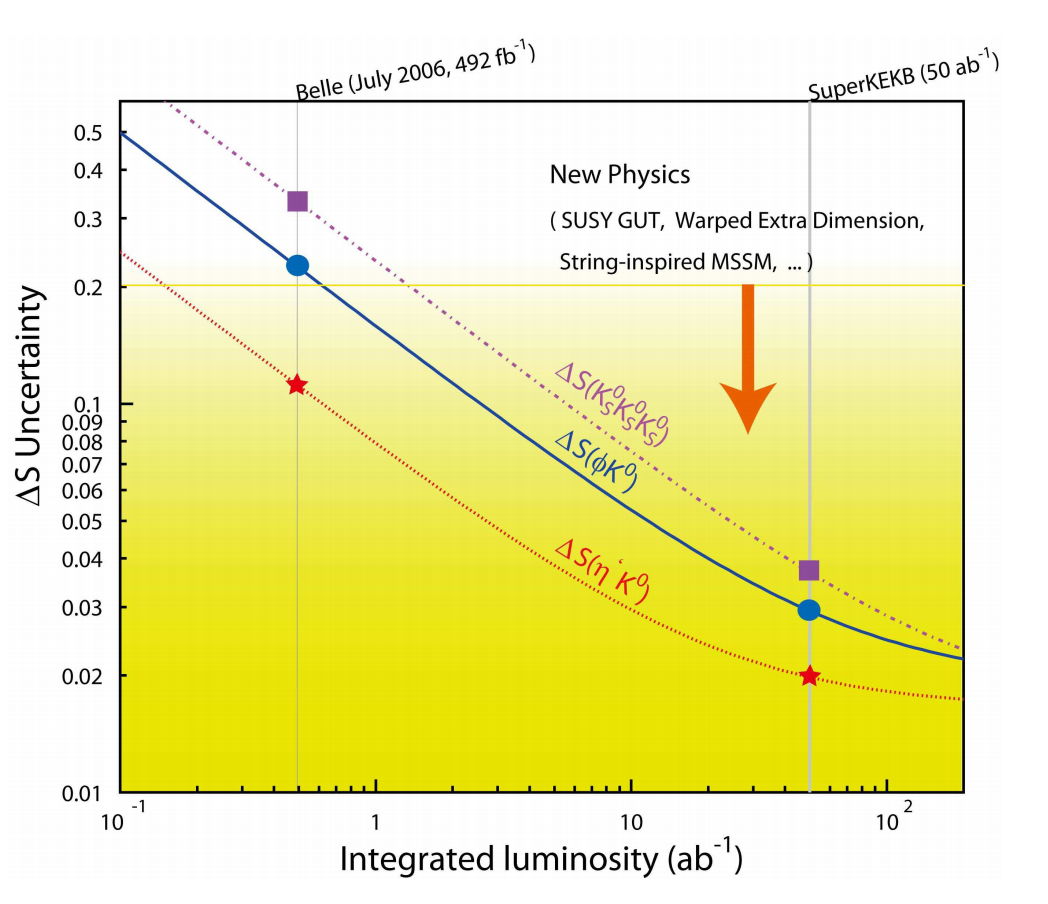
\includegraphics[height=10cm]{sensitivity}
	\caption{Expected  sensitivity of $\Delta \mathcal{S}$ regarding the integrated luminosity of Belle II prospective.\cite{Abe:2010gxa}}
	\label{fig:sensitivity}
\end{figure}

\begin{table}[H]
	\centering
	\large
	\caption{$\Delta \mathcal{S}$ scaled uncertainty (statistical) with integral luminosity \cite{Abe:2010gxa}.}
	\label{tab:sensitivity}
	\begin{tabular}{c c c c}
		\toprule
		Observable & Belle ($0.5 \: \text{ab}^{-1}$) & Belle II ($5 \: \text{ab}^{-1}$)& Belle II ($50 \: \text{ab}^{-1}$)\\
		\hline
		$\Delta \mathcal{S}_{\phi K^0_S}$ & 0.22 &  0.073 & 0.029\\
		$\Delta \mathcal{S}_{\eta' K^0_S}$   & 0.11 &  0.038 & 0.020\\
		$\Delta \mathcal{S}_{ K^0_S K^0_S K^0_S}$ & 0.33 & 0.105 & 0.037\\
		\bottomrule
	\end{tabular}
\end{table}

\begin{comment}
As the main decay process that have been studied in this thesis, $B^0_d\to K^0_S K^0_S K^0_S$ propagates through $b\to \bar{s}ss$ as well. There are more than one process that will yield the same final states ($3K_S^0$). The difference here is that $3K_S^0$ final states can be produced not only from the $ss$ intermediate state like $f_0(980)$ through penguin mode, but also viable from charm decay (see Fig(1-10)), which $\bar{c}c$ comes from tree level transition. The contribution from tree level process is estimated to be small but must be aware of using Dalitz analysis in future. Similarly, the $\bar{s}s$ intermediate decay, such as $B^0 \to f_0(980)K^0_S$, would also give the same $\it{CP}$-eigenvalue in final states, which is also considered as signal because of $\it{CP}$-even), while $b\to c\to s$ tree level is considered as background that yields $\it{CP}$-odd final states. The previous result in this channel from Belle full dataset \cite{kang2020measurement} is:  $\mathcal{S}$ = -sin2$\phi_1$ = $-0.72\pm 0.23(stats)\pm 0.05(syst)$ and $\mathcal{A}=0.12\pm0.16(stats)\pm 0.05(syst)$. The earlier results from Babar\cite{lees2012amplitude} is: $\mathcal{S}$ = -sin2$\phi_1$ = $-0.94^{+0.21}_{-0.24}(stats)\pm 0.06(syst)$. The results are mostly limited by the statistical uncertainty with minor difference. With the expected luminosity from Belle II in future, we are able to cut off the margin in between the results and the Standard Model. This thesis, as the first trial to perform the $\it{CP}$ measurement on this channel for Belle II, is inevitably dominated by the low data size in the early operation, but will show the good capability and potential in the analysis tools and methods towards the promising future.
\end{comment}

% 2021.01.26 ends move below to the chapter 3

\begin{comment}
\begin{figure}[h]
\begin{minipage}[t]{0.33\linewidth} % 如果一行放2个图,用0.5,如果3个图,用0.33
\centering 
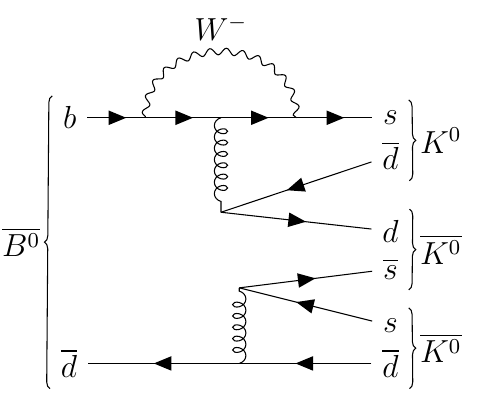
\includegraphics[height=4cm]{feynman3Ks01} 
\label{fig:side:a} 
\end{minipage}%
\begin{minipage}[t]{0.33\linewidth} 
\centering 
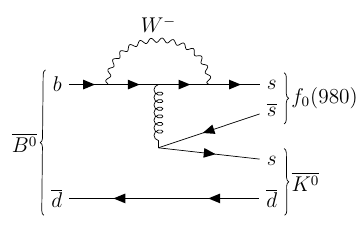
\includegraphics[height=4cm]{feynman3Ks02} 
%\caption{ } 
\label{fig:side:b} 
\end{minipage}% 
\begin{minipage}[t]{0.33\linewidth} 
\centering 
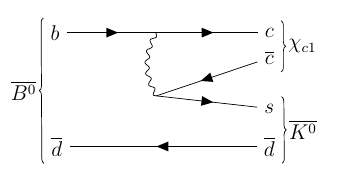
\includegraphics[height=3cm]{feynman3Ks03} 
%\caption{ } 
\label{fig:side:a} 
\end{minipage} %
\caption{non-resonant signal (left),resonant signal (middle) and tree-level resonant backgrounds (right)
$B^0_d\to3K^0_S$ diagrams}.
\end{figure}
\end{comment}



\begin{comment}
\begin{tikzpicture}
\begin{feynman}
\vertex (a1) {\( b\)};
%\vertex[right=1cm of a1] (a2);
\vertex[right=2cm of a1] (a3);
%\vertex[right=1cm of a3] (a4) ;
\vertex[right=2cm of a3] (a5) {\(c\)};
\vertex[below=1.25cm of a3] (a6) ;
\vertex[below=0.5cm of a5] (a7) {\(\overline{c}\)};
\vertex[below=1.5cm of a5] (a8) {\(s\)};
\vertex [below=0.75cm of a8] (b1) {\(\overline{d}\)};
%\vertex [left=2cm of b1] (b2);
\vertex [left=4.2cm of b1] (b3) {\(\overline{d}\)};
%\vertex [above=1cm of b2] (b4);
%\vertex [above=0.5cm of b1] (b5) {\({s}\)};
%\vertex [above=1.25cm of b1] (b6) {\(\overline{s}\)};
\diagram*{
{[edge=fermion],
(a1)--(a3)--(a5),
(b1)--(b3),
(a7)--(a6)--(a8),
%(b5)--(b4)--(b6),
},
%(b2)--[gluon] (b4),
(a3)--[photon, bend right] (a6),
%(a2)--[boson, half left,edge label=\(W^{-}\)] (a4)
};
\draw [decoration={brace}, decorate] (b3.south west) -- (a1.north west)
node [pos=0.5, left] {\(\overline{B^{0}}\)};
\draw [decoration={brace}, decorate]  (a8.north east)--(b1.south east) node [pos=0.5, right] {\(\overline{K^{0}}\)};
\draw [decoration={brace}, decorate]  (a5.north east)--(a7.south east) 
node [pos=0.5, right] {\(\chi_{c1}\)};
%\draw [decoration={brace}, decorate]  (a8.north east)--(b6.south east) 
%node [pos=0.5, right] {\(\overline{K^{0}}\)};
\end{feynman}
\end{tikzpicture}
\end{comment}
